\chapter{Sanskrit conjugation}

Implementing verbal inflection or conjugation in the Sanskrit module is the most difficult task. The main reason is there are no complete lists of verbal paradigms in Sanskrit because many verb forms never came into use and finite verbs became less in use by replacements of non-finite/derivative verb forms. That is to say, what you shall see in conjugation tables is to some extent a theoretical speculation.

Like the tools for declension, we have two related tools for conjugation: \emph{Verbal Paradigms} and \emph{Conjugation Table}

\section{Verbal Paradigms}

Much like Nominal Paradigms as you have seen in the last chapter, this tool lists all known verbal paradigms. When you first open the tool by menu Sanskrit > {\faSix \symbol{"F5BF}} Verbal Paradigms, you will see the paradigm table with the following information:

\begin{compactenum}
\item Name of the paradigm, usually identical to the prathama (3rd person) singular conjugation of the sample verb
\item Reference to tables in Bucknell's Manual\footnote{This column can be empty in some entries. This means the paradigm is taken from another source, particularly Madhav M.\ Deshpande's \emph{Saṃskṛtasubhodhinī: A Sanskrit Primer} (2007, University of Michigan), if not a speculation of the author alone.}
\item Tense/Mood, named after Bucknell's Manual
\item Pada, either Active form (\pali{parasmaipada}) or Middle form (\pali{ātmanepada})
\item Prathama Samples, i.e., prathama (3rd person) singular, dual, and plural of the conjugation
\end{compactenum}

When a row is clicked, the full table of that paradigm will be shown at the bottom. The list on the right shows all words rendered, normally ordered (in contrast with the list of nominal paradigms, which is ordered by endings). Figure \ref{fig:sanskrit-verbparad} shows what has been described so far.

\begin{figure}[!hbt]
\centering
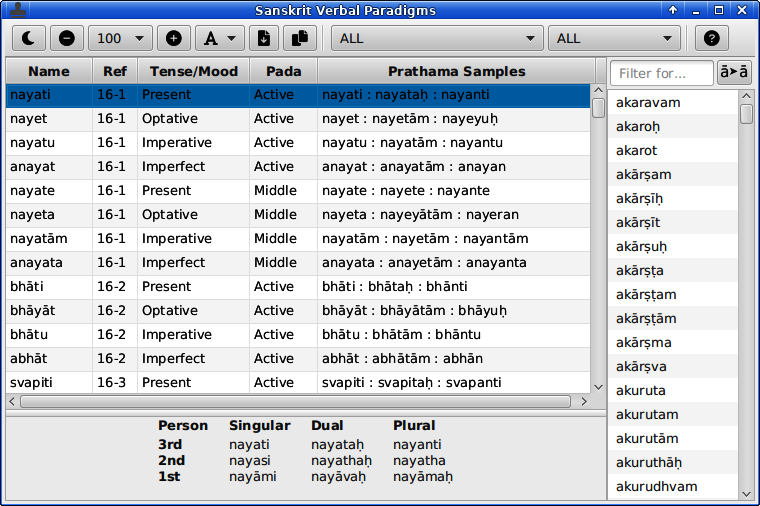
\includegraphics[width=0.9\linewidth]{images/sanskrit-verbparad.png}\\
\caption{Window of Verbal Paradigms}
\label{fig:sanskrit-verbparad}
\end{figure}

You can select only a specific tense or mood by the selector in the tool bar, as well as only active (\pali{parasmaipada}) or middle (\pali{ātmanepada}) form by its selector nearby. By default, both selectors are set to ALL. Figure \ref{fig:sanskrit-verbperf} shows results only of perfect tense with active verb form. Note that not all tenses and moods have paradigms. Some use related paradigms with a modified stem. For example, conditional mood uses future stems with imperfect paradigms. And when a specific tense or mood is selected, the word list on the right is changed accordingly.

\begin{figure}[!hbt]
\centering
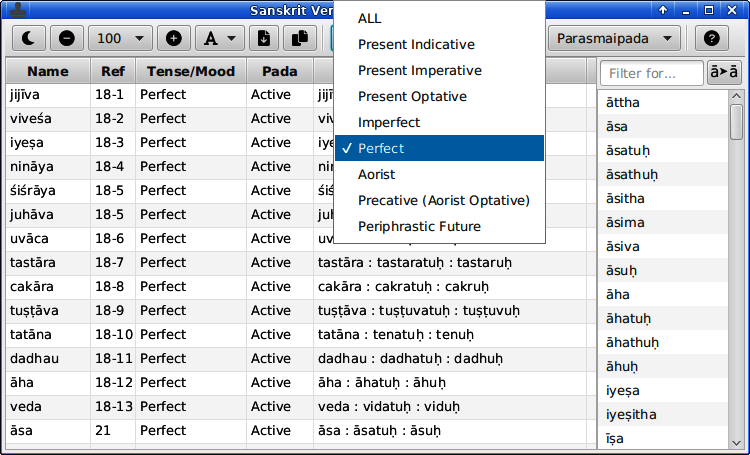
\includegraphics[width=0.9\linewidth]{images/sanskrit-verbperf.png}\\
\caption{Selection only active perfect paradigms}
\label{fig:sanskrit-verbperf}
\end{figure}

\section{Conjugation Table}

This is the most complicated tool of all. Behind the tables you shall see, a lot of energy and time have been used in the production. The ideal goal of this tool is all roots/verbs should be listed and be able to select, then renditions of all verb forms should be seen. The ideal goal is definitely infeasible. However, if we target only \emph{some} roots/verbs and \emph{some} verb forms, instead of \emph{all} of them, the function are possible to be implemented.

Good news is Bucknell has listed 433 common verbs in his Manual\footnote{There are 432 root plus \pali{adhi +} \paliroot{i}.}, but bad news is just around 20 verbs so far that can be rendered fully to all applicable forms in this tool. The complete task of the addition is so laborious that it may be finished in the far future, if it is able to be done at all. However, even though not all verbs are completed, we have the full list of them and at least the rendition into present verb forms is available.

Conjugation Table can be opened by menu Sanskrit > {\faSix \symbol{"F00A}} Conjugation Table. There are two modes of display: (1) for main or finite verb forms, enabled by {\faSix M} button (default), and (2) derivative verb forms, enabled by {\faSix D} button. Figure \ref{fig:sanskrit-conjugtable} shows a finite verb with present indicative selected.

\begin{figure}[!hbt]
\centering
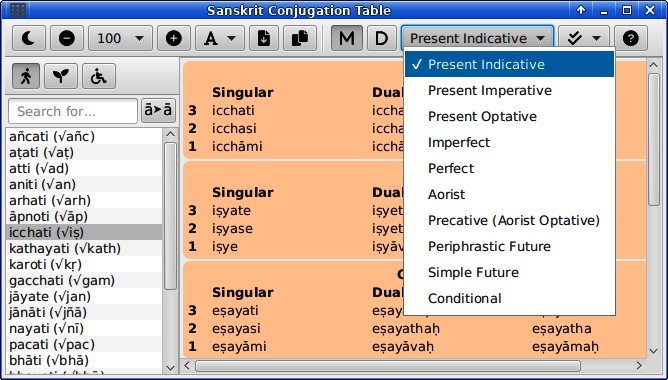
\includegraphics[width=0.9\linewidth]{images/sanskrit-conjugtable.png}\\
\caption{Verb form selector in Conjugation Table}
\label{fig:sanskrit-conjugtable}
\end{figure}

The left pane is the list of words to be selected. On the top of the pane, there is its tool bar with three toggle buttons and a text field for searching. The first two buttons list verbs that can be rendered in all forms, but with different display. The button {\faSix \symbol{"F554}} shows verbs by their citation form with root (see Figure \ref{fig:sanskrit-conjugtable}), e.g., \pali{icchati} (\paliroot{iṣ}), whereas the button {\faSix \symbol{"F4D8}} shows by their root, class, meaning, and Bucknell's number, e.g., \paliroot{iṣ} 6 desire [18]. All verbs/roots are ordered by Bucknell's number.\footnote{Bucknell gives each verb a number, running from 1 to 432, ordered by root's name. The last one is \pali{adhi +} \paliroot{i} (\pali{adhīte}) having \emph{16a} as its number.} Figure \ref{fig:sanskrit-conjug-icchati} shows a selection by root's name when the second button is enabled

\begin{figure}[!hbt]
\centering
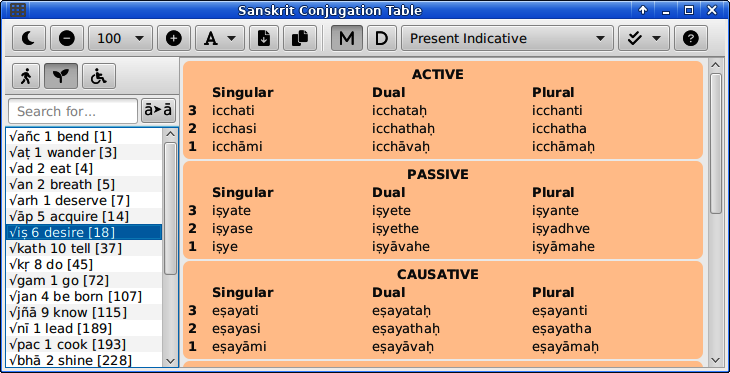
\includegraphics[width=0.9\linewidth]{images/sanskrit-conjug-icchati.png}\\
\caption{Conjugation of \pali{icchati} selected by root's name}
\label{fig:sanskrit-conjug-icchati}
\end{figure}

The last button ({\faSix \symbol{"F193}}), when enabled, all the rest of verbs are listed, with the format of the previous two combined. Verbs in this list, as illustrated by the icon, are lame. They can be rendered to certain forms, largely to tenses and moods that use the present stem, i.e., present, imperative, optative, and imperfect, except \paliroot{ah} that has only some perfect forms (\pali{āha}, for example, see Figure \ref{fig:sanskrit-conjug-say}).\footnote{In the future, this `lame' list should be decreased in number, and we will have more complete verbs.}

The finding of a verb/root is simple. You just enter some word or part of it in the text field, then the information in the list is searched (in any parts). Figure \ref{fig:sanskrit-conjug-say} shows results of a search for `say'. In those, you also see \pali{vāsayati} which also has `say' in the word. If you want to know what else means `say', it is better to search for `speak' as well.

\begin{figure}[!hbt]
\centering
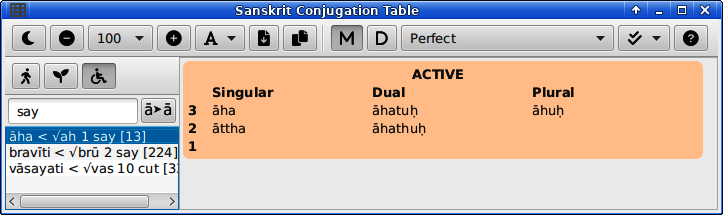
\includegraphics[width=0.9\linewidth]{images/sanskrit-conjug-say.png}\\
\caption{Search results for `say'}
\label{fig:sanskrit-conjug-say}
\end{figure}

Showing derivative verb forms in the tool has similar functions, but instead of having tense/mood selector we have derivative form selector here. Figure \ref{fig:sanskrit-conjugderi} shows perfect passive participle of \pali{icchati}. Remember that the output of derivative verbs is mostly adjectives, so we will see declension tables of the three genders in the result area. However, some verb forms have indeclinable output, i.e., infinitive and absolutive.

\newpage
\begin{figure}[!hbt]
\centering
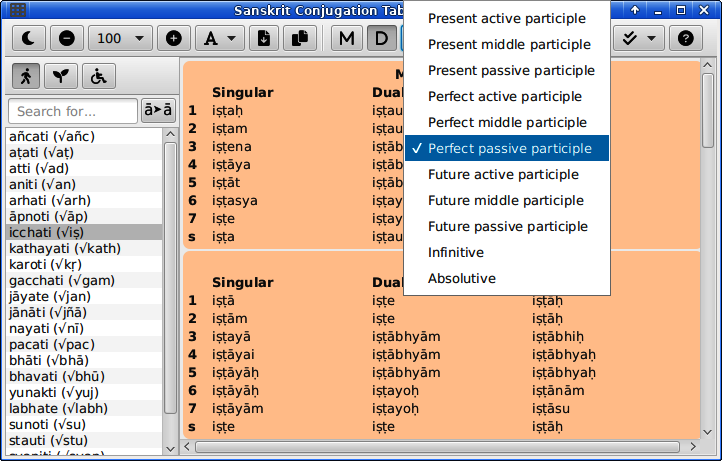
\includegraphics[width=0.9\linewidth]{images/sanskrit-conjugderi.png}\\
\caption{Derivative verb form selector}
\label{fig:sanskrit-conjugderi}
\end{figure}

If you need Devanāgarī output, you can enable its option like we do in Declension Table. For other minor details, you have to learn the tool by playing with it. As for the verb system in Sanskrit is the heart of the grammar, mastering this tool will help you master the language easier.
